% XeLaTeX

\documentclass{article}
\usepackage{ctex}
\usepackage{xypic}
\usepackage{amsfonts,amssymb}
\usepackage{multirow}
\usepackage{geometry}
\usepackage{graphicx}
\usepackage{listings}
\usepackage{lipsum}
\usepackage{courier}
\usepackage{fancyvrb}
\usepackage{etoolbox}


\linespread{1.2}
\geometry{left=3cm,right=2.5cm,top=2.5cm,bottom=2.5cm}

\makeatletter
\patchcmd{\FV@SetupFont}
  {\FV@BaseLineStretch}
  {\fontencoding{T1}\FV@BaseLineStretch}
  {}{}
\makeatother

\lstset{basicstyle=\small\fontencoding{T1}\ttfamily,breaklines=true}
\lstset{numbers=left,frame=shadowbox,tabsize=4}
%\lstset{extendedchars=false}
\begin{document}

\title{实验六 \ 多进程操作系统 \ 实验报告}
\author {数据科学与计算机学院 \ 计算机科学与技术 2016 级 \\ 王凯祺 \ 16337233}
\maketitle

\section{实验目的}

\begin{itemize}
\item 在内核实现多进程的二状态模,理解简单进程的构造方法和时间片轮转调度过程。
\item 实现解释多进程的控制台命令,建立相应进程并能启动执行。
\item 至少一个进程可用于测试前一版本的系统调用,搭建完整的操作系统框架,为后续实验项目打下扎实基础。
\end{itemize}

\section{实验要求}

保留原型原有特征的基础上,设计满足下列要求的新原型操作系统:

\begin{itemize}
\item 在 C 程序中定义进程表,进程数量至少4个。
\item 内核一次性加载多个用户程序运行时,采用时间片轮转调度进程运行,用户程序的输出各占1/4屏幕区域,信息输出有动感,以便观察程序是否在执行。
\item 在原型中保证原有的系统调用服务可用。再编写1个用户程序,展示系统调用服务还能工作。
\end{itemize}

\section{特别声明}

\begin{itemize}
\item 为了让屏幕输出更简洁、代码更精简,我决定删去上一实验中原有的 8h 时钟中断的所有功能;本实验的 8h 时钟中断将实现新功能——进程切换。
\item 由于本实验中内核和用户程序都作为进程,进行时间片轮转,改写 9h 中断(输出 ouch!)会影响内核调用 16h 中断读取字符,我决定不使用上一实验中改写的 9h 中断,用回 BIOS 的 9h 中断。
\end{itemize}

\section{实验步骤}

\subsection{设计思路}

引导程序启动后加载内核,并把内核视为一个进程,并为其创建进程控制块,并将该进程控制块记为“运行”。

时钟中断响应后,保存当前进程 A 的寄存器状态,并将进程 A 的进程控制块记为“就绪”;寻找下一个进程 B ;还原进程 B 的寄存器状态,并将 B 的进程控制块记为“运行”。

\subsection{设计进程控制块}

首先要明确:需要保存多少个寄存器。我在 MASM 6.1 指引手册(见“参考资料”文件夹)第 54 页至 57 页找到了答案。 8086 计算机有以下寄存器:

\begin{itemize}
\item 主寄存器: AX, CX, DX, BX, SP, BP, SI, DI
\item 段寄存器: DS, ES, SS, CS
\item 指令指针寄存器: IP
\item 标志寄存器
\end{itemize}

我计划使用 C 的结构体来保存进程控制块。

now\_process 表示当前正在运行的进程。

alive 表示进程是否还活着。若 PCBlist[i].alive = 1 且 $now\_process = i$ ,则表示 $i$ 进程处于“运行”状态;若 PCBlist[i].alive = 1 且 $now\_process \neq i$ ,则表示 $i$ 进程处于“就绪”状态。

\begin{lstlisting}[language=C]
typedef struct PCB {
	int ax;
	int bx;
	int cx;
	int dx;
	int si;
	int di;
	int bp;
	int es;
	int ds;
	int ss;
	int sp;
	int ip;
	int cs;
	int flags;
	int alive;
	char pname[16];
};

struct PCB PCBlist[64];

int now_process;
\end{lstlisting}

PCBlist 的下标即代表进程号,同时也代表进程在磁盘中的扇区号。虽然这样的管理模式下无法为一个程序创建两个进程,但是此模式编程复杂度低,并且简单易懂。

\subsection{设计 Save 过程和 Restart 过程}

我在 MASM 6.1 指引手册 第 92 页找到了中断发生的工作原理。中断发生时,由 CPU 将标志寄存器 Flags 、代码段寄存器 CS 、指令指针寄存器 IP \textbf{依次}压入堆栈(被中断的程序的堆栈);中断返回时(即执行 iret 指令时),CPU 将堆栈中的指令指针寄存器 IP 、代码段寄存器 CS 、标志寄存器 Flags \textbf{依次}弹出堆栈,并转到 CS:IP 继续原程序的执行。

照着文档,我读懂了老师提供的“现场保护:save过程(旧版)”代码和“现场恢复:restart过程(旧版)”代码。老师的代码全都加了注释,我要给老师点个大大的赞!

我计划 Schedule 过程由 C 实现,故 save 过程只需将寄存器保存在外部变量(C 语言的变量),然后 Restore 过程需要将外部变量还原到寄存器中。如此安排,Schedule 过程要做的事情是:将 C 语言的变量保存到 A 进程控制块中,然后调度另一进程 B ,将 B 进程控制块中的寄存器写入 C 语言的变量。

以下是外部变量的声明:

\begin{lstlisting}[language={[x86masm]Assembler}]
extrn _ax_save:word
extrn _bx_save:word
extrn _cx_save:word
extrn _dx_save:word
extrn _si_save:word
extrn _di_save:word
extrn _bp_save:word
extrn _es_save:word
extrn _ds_save:word
extrn _ss_save:word
extrn _sp_save:word
extrn _ip_save:word
extrn _cs_save:word
extrn _flags_save:word
\end{lstlisting}

以下是 save 过程代码(MASM 格式):

\begin{lstlisting}[language={[x86masm]Assembler}]
	push ds					; StackTop: *\flags\cs\ip\ds(user)
	push cs					; StackTop: *\flags\cs\ip\ds(user)\cs(kernel)
	pop ds					; StackTop: *\flags\cs\ip\ds(user)
							; ds <- kernel cs
	mov _ax_save, ax		; Save ax
	pop ax					; StackTop: *\flags\cs\ip
							; ax <- ds(user)
	mov _ds_save, ax		; Save ds
	pop ax					; StackTop: *\flags\cs
	mov _ip_save, ax		; Save ip
	pop ax					; StackTop: *\flags
	mov _cs_save, ax		; Save cs
	pop ax					; StackTop: *
	mov _flags_save, ax		; Save flags
	
	mov _bx_save, bx		; Save bx
	mov _cx_save, cx		; Save cx
	mov _dx_save, dx		; Save dx
	mov _si_save, si		; Save si
	mov _di_save, di		; Save di
	mov _bp_save, bp		; Save bp
	mov ax, es
	mov _es_save, ax		; Save es
	mov ax, ss
	mov _ss_save, ax		; Save ss
	mov _sp_save, sp		; Save sp
\end{lstlisting}

以下是 restart 过程代码(MASM 格式):

\begin{lstlisting}[language={[x86masm]Assembler}]
	mov sp, _sp_save		; Restore sp
	mov ax, _ss_save
	mov ss, ax				; Restore ss
	mov ax, _es_save
	mov es, ax				; Restore es
	mov bp, _bp_save		; Restore bp
	mov di, _di_save		; Restore di
	mov si, _si_save		; Restore si
	mov dx, _dx_save		; Restore dx
	mov cx, _cx_save		; Restore cx
	mov bx, _bx_save		; Restore bx
	mov ax, _flags_save
	push ax					; Restore flags
	mov ax, _cs_save
	push ax					; Restore cs
	mov ax, _ip_save
	push ax					; Restore ip
	mov ax, _ds_save
	push ax
	mov ax, _ax_save		; Restore ax
	pop ds					; Restore ds
\end{lstlisting}

\subsection{设计 Schedule 过程}

\subsubsection{设置数据段、栈指针}

Schedule 过程应位于 Save 过程和 Restart 过程之间。

Save 过程和 Restart 过程没有访问数据段也能正确运行,但 Schedule 过程要存取进程控制块,必须设置正确的数据段才能正确运行。为了避免与其他用户程序冲突,我精心设置了 Schedule 过程使用的栈指针。

\begin{lstlisting}[language={[x86masm]Assembler}]
	mov ax, 0a00h
	mov ds, ax
	mov es, ax
	mov ss, ax
	mov sp, 100h
\end{lstlisting}

\subsubsection{时间片轮转}

时间片轮转即是从下一个编号开始,逐个查询程序状态。若该程序“就绪”,就跳转到该程序。

\begin{lstlisting}[language=C]
	now_process = (now_process + 1) % 64;
	while (!PCBlist[now_process].alive)
		now_process = (now_process + 1) % 64;
\end{lstlisting}

在这里,我栽了一个跟头:在完成了时间片轮转之后,我把内核挂到虚拟机运行,发现两个有趣的现象:

\begin{itemize}
\item 如果不碰键盘,时钟中断以每秒 18.2 次的速度不断运行
\item 一旦碰了键盘,时钟中断下一次响应后卡死
\end{itemize}

我怀疑是 Save 过程和 Restart 过程有误,在屏幕上输出了这些寄存器的值,发现都是正确的值。

\begin{figure}[!hbp]
	\centering
	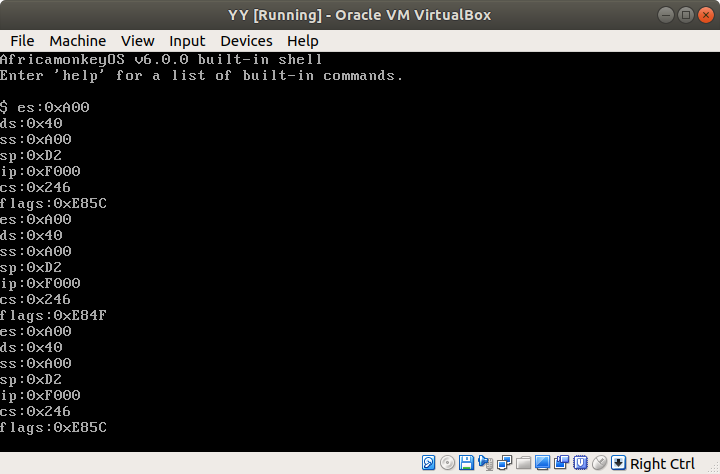
\includegraphics[scale=0.55]{pics/1.png}
\end{figure}

同时我也怀疑是不是 Flags 是 8 位而不是 16 位的,经查询文档,此处无错。

经吴梓阳同学指点,我下载了 Bochs 并用 bochsdbg 调试。我设置了两个断点,一个是 Save 过程前,一个是 Restore 过程后。

我用 r 指令查看了寄存器的值,前后一致。再用 print-stack 指令查看了堆栈的值,只有栈顶指针和栈顶的 Flags, CS, IP 一致,其他的全都变了!

堆栈被篡改,我认为一定是 16h 中断把堆栈中的元素改了。再继续跟踪发现,根本不是 16h 的问题。Kernel 进程的 ss:sp 为 0a00:0100 ,而我 Schedule 过程的 ss:sp 也为 0a00:0100 。在执行 Schedule 的过程中,会修改 Kernel 进程的栈中元素的值。亏我还精心设置 ss:sp ,居然把 Kernel 给忘记了……

我将 Schedule 的 ss:sp 设置为 0a00:0000 ,问题解决!

\newpage

下图为用 Bochs 调试的过程,截图为 Save 过程前的寄存器/堆栈状态。

\begin{figure}[!hbp]
	\centering
	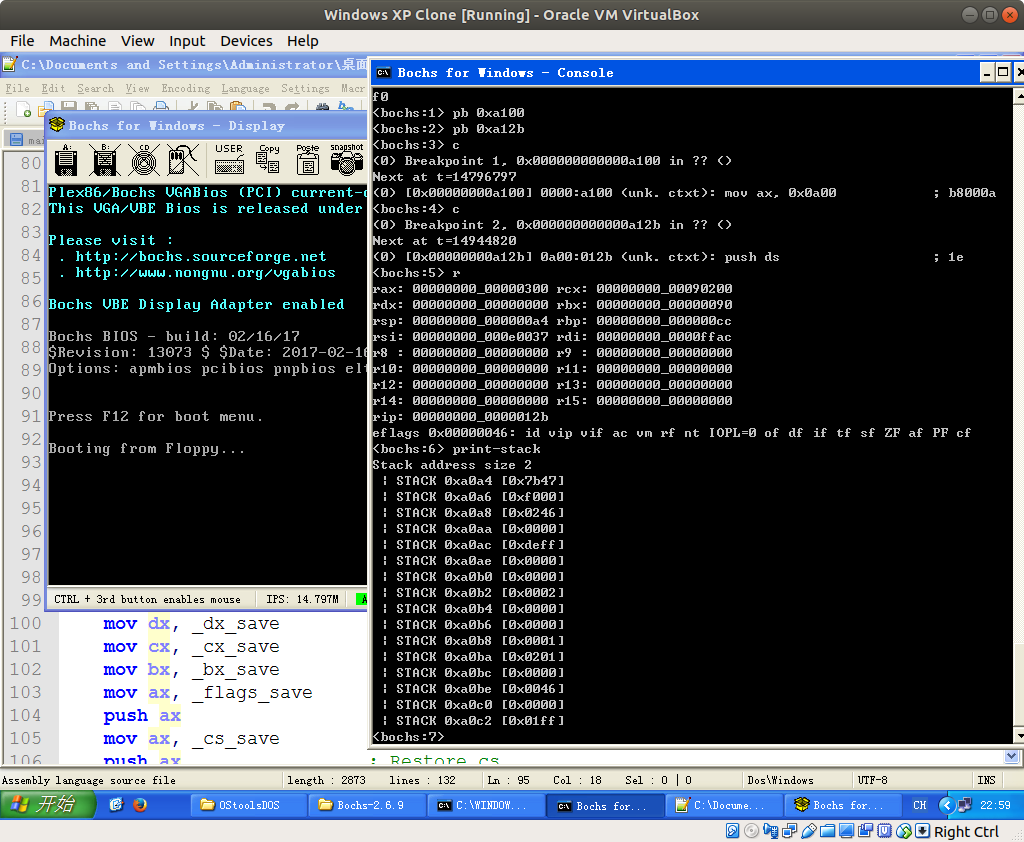
\includegraphics[scale=0.4]{pics/2.png}
\end{figure}

\subsubsection{创建新进程}

我的思路是:首先创建进程控制块,将 cs, ds 等寄存器设置为合适的值,然后设置该进程为“就绪”状态。考虑到进程结束后应返回内核并将该进程的 alive 属性设置为 0 ,操作系统应事先在其用户栈内写入返回 cs 和返回 ip 。用户程序返回内核后,将 alive 属性设置为 0 ,死循环等待时钟中断发生。时钟中断发生后,该进程结束,下一次时间片轮转将不再轮到它。

下面是我在 main.c 中创建新进程的代码片段:

\begin{lstlisting}[language=C]
	if (PCBlist[pid].alive) {
		puts("error: This program is running");
		return;                  /* 不支持同一个程序创建两个进程 */
	}
	clear_new_pcb();             /* 清空 pcb */
	cs1 = 0x2000 + 0x40 * pid;   /* 新进程加载点 cs */
	ip1 = 0x100;                 /* 新进程加载点 ip */
	new_pcb.cs = cs1;
	new_pcb.ds = cs1;
	new_pcb.es = cs1;
	new_pcb.ss = cs1;
	new_pcb.ip = ip1;
	new_pcb.sp = ip1 - 6;        /* 预留空间写入返回cs,返回ip,以及当前pid */
	new_pcb.flags = 512;         /* IF = 1 */
	
	asm mov cx, ds
	asm push ds
	asm mov ax, cs1
	asm mov ds, ax
	asm mov bx, ip1
	asm sub bx, 2
	asm mov al, pid
	asm mov ah, 0
	asm mov [bx], ax             /* 将进程编号压入用户堆栈 */
	asm sub bx, 2
	asm mov ax, cx
	asm mov [bx], ax             /* 将返回 cs 压入用户堆栈 */
	asm sub bx, 2
	asm mov ax, offset exe_go
	asm mov [bx], ax             /* 将返回 ip 压入用户堆栈 */
	asm pop ds
	
	make_alive(pid);             /* 将进程控制块记为“就绪” */
	execute(pid, cs1, ip1);      /* 从磁盘拷贝程序到内存中 */
	asm exe_go:
	asm mov ax, 0a00h
	asm mov ds, ax
	asm mov es, ax
	if (now_process == 0) return;/* 识别 fork 后是内核还是用户程序 */
	asm pop ax                   /* 从栈提取进程编号 */
	asm mov pid, al
	make_die(pid);               /* 删除进程控制块 */
	asm jmp $                    /* 死循环,让这个程序自生自灭吧 :) */
\end{lstlisting}

这里面也发生了一些有趣的状况:程序退出后没有返回到内核,也就是说没有修改进程控制块的状态。

用 Bochs 跟踪后发现,第 29 行结束后 ax 的值是 0x0159 ,而 cs 为 0 ,怪不得跳不回内核啦!查文档知 offset 是针对于 COM 开头的偏移量,而不是针对 cs 的偏移量。所以,应该将 ds 作为 cs 压入堆栈,将 offset 作为 ip 压入堆栈。

\subsection{设计 top 命令}

top 命令可以显示当前活动的所有进程,遍历进程控制块后输出即可。

\begin{lstlisting}[language=C]
void print_top() {
	int i, k;
	puts("=============================");
	puts("Process ID | Process Name    ");
	puts("-----------------------------");
	for (i = 0; i < 64; ++i)
		if (PCBlist[i].alive) {
			printint_format(i, 10);
			puts_no_new_line(" | ");
			puts(PCBlist[i].pname);
		}
	puts("=============================");
}
\end{lstlisting}

\subsection{设计 kill 命令}

kill 命令可以用于结束进程。我们可以遍历进程控制块,找到该进程并将其 alive 置 0 。则以后时间片轮转就不再轮到它,从而实现结束进程。

\begin{lstlisting}[language=C]
void kill_process() {
	int pid, i, j;
	pid = 0;
	for (i = 4; cmd[i]; ++i)
		if (cmd[i] >= '0' && cmd[i] <= '9') {
			for (j = i; cmd[j] >= '0' && cmd[j] <= '9'; ++j) {
				pid = pid * 10 + cmd[j] - '0';
				if (pid >= 64) {
					puts("Process not found");
					return;
				}
			}
			if (pid == 0) {
				puts("Kernel process can not be killed");
				return;
			}
			if (PCBlist[pid].alive == 0) {
				puts("Process not found");
				return;
			}
			PCBlist[pid].alive = 0;
			puts_no_new_line("Process ");
			printint_format(pid, 0);
			puts(" killed");
			return;
		} else
		if (st[i] >= 33) {
			puts("Usage: kill PID");
			return;
		}
	puts("Usage: kill PID");
}
\end{lstlisting}

\section{操作系统使用说明书}

\subsection{help 命令}

输入命令 help ,即可查看操作系统支持的所有命令。

\begin{figure}[!hbp]
	\centering
	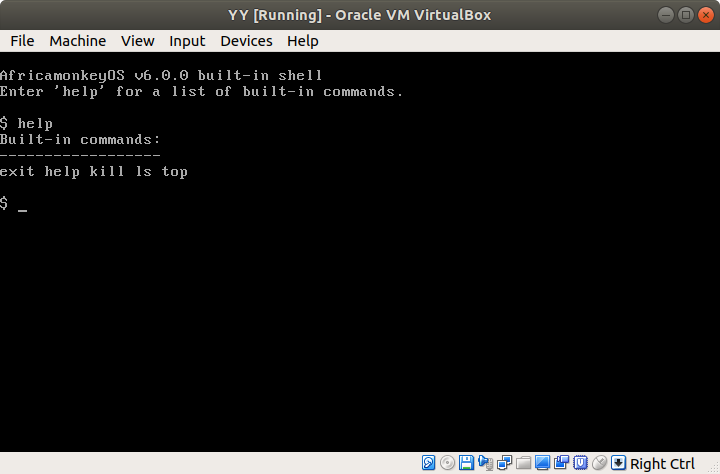
\includegraphics[scale=0.5]{pics/3.png}
\end{figure}

\subsection{ls 命令}

输入命令 ls ,即可查看操作系统内的程序。操作系统会显示每个程序的文件名,扇区编号和程序大小。

\begin{figure}[!hbp]
	\centering
	
\includegraphics[scale=0.5]{pics/4.png}
\end{figure}

\newpage

\subsection{执行程序}

在 ls 命令中,可以查询到程序的文件名。输入文件名即可运行程序。

运行程序将会创建一个新的进程,内核仍可响应命令。

依次键入下面的命令,每敲击一个命令,就会创建一个新进程,执行相应的用户程序。4 条命令键入完毕后,将会看到 4 个程序以时间片轮转的方式执行。

\begin{lstlisting}
a
bc
def
1234
\end{lstlisting}

\begin{figure}[!hbp]
	\centering
	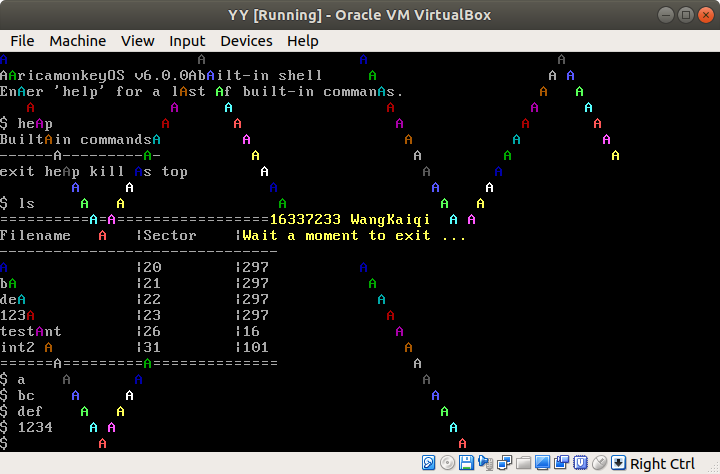
\includegraphics[scale=0.5]{pics/5.png}
\end{figure}

\subsection{top 命令}

top 命令可查看当前操作系统正在运行的进程。

下图中,我执行了 a 和 bc 两个用户程序。输入 top 命令,可以看到有 3 个进程在运行,它们分别是: 0 号进程,操作系统内核 kernel;20 号进程,用户程序 a;21 号进程,用户程序 bc 。

\newpage

\begin{figure}[!hbp]
	\centering
	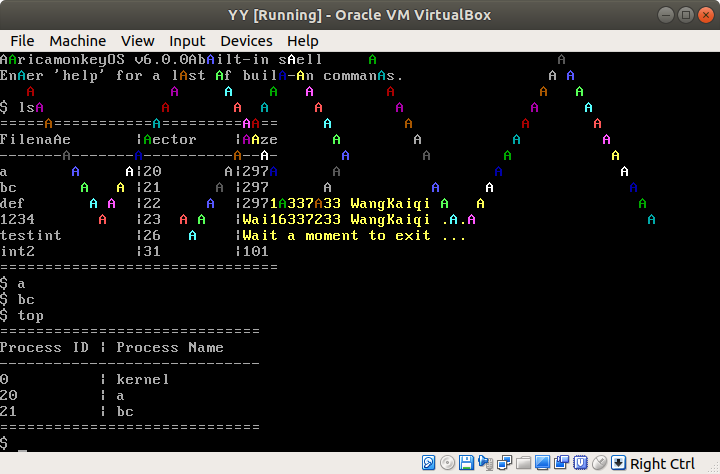
\includegraphics[scale=0.5]{pics/6.png}
\end{figure}


\subsection{kill 命令}

kill 命令可杀死一个进程,用法: kill 进程编号。

下图中,我想终止第一个用户程序(进程号 20,文件名为 a),则输入 kill 20 ,内核会返回 Process 20 killed ,即成功杀死进程 20 。

\begin{figure}[!hbp]
	\centering
	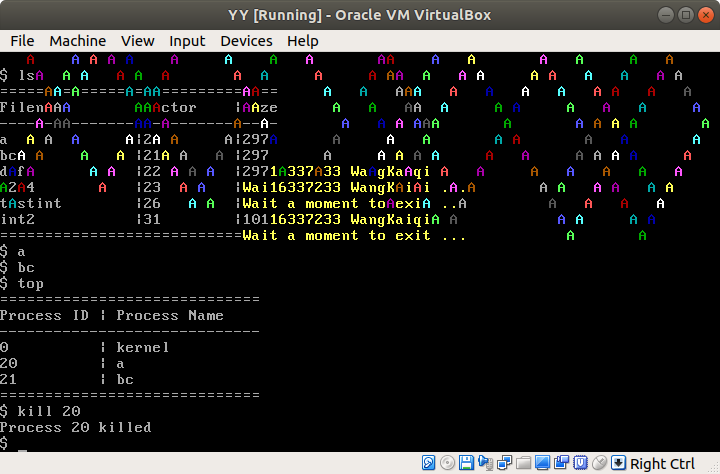
\includegraphics[scale=0.5]{pics/7.png}
\end{figure}

\section{实验总结}

这次实验让我深入了解了多进程时间片轮转的工作原理。原理很简单,就是 Save, Schedule 和 Restart ,但实现起来可不简单。

在 Save 过程和 Restart 过程中,最容易出错是栈。当前栈内元素是什么,这个一定要非常清楚。当使用 call 操作和 ret 操作时,会修改堆栈。所以 Save 过程和 Restart 过程应尽量避免使用 call 和 ret 操作,避免出错。另外, ss 和 sp 的保存时机也是非常关键的。ss 和 sp 必须在最后保存,这样做是为了保存弹出 flags, cs, ip 之后的栈指针。

在 Schedule 过程中,更容易在栈的问题上出错。 Schedule 的栈要与 Kernel 的栈以及用户程序的栈都不一样,否则会覆盖原有的数据。一旦踩进这个坑,就很难跳出来,因为你会发现寄存器之类的全部都是对的,只有栈内元素是错的。 Bochs 真的是一个很好的调试工具,帮助我看到栈内元素是错误的,让我跳出这个坑。



\end{document}
















